\documentclass{standalone}
\usepackage{tikz}
\usepackage{pgfplots}
\pgfplotsset{compat=1.18}
\usepgfplotslibrary{fillbetween}

\begin{document}
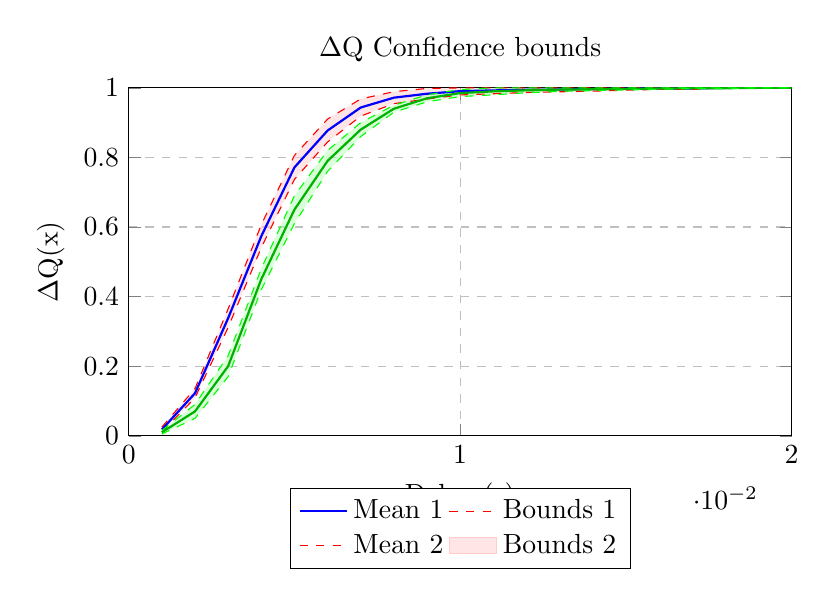
\begin{tikzpicture}
\begin{axis}[
    title={$\Delta$Q Confidence bounds},
    xlabel={Delay (s)},
    ylabel={$\Delta$Q(x)},
    xmin=0, xmax=0.02,
    ymin=0, ymax=1,
    xtick={0,0.01,0.02},
    ytick={0,0.2,0.4,0.6,0.8,1},
    ymajorgrids=true,
    xmajorgrids=true,
    grid style=dashed,
    width=10cm,
    height=6cm,
    legend style={at={(0.5,-0.15)}, anchor=north, legend columns=2},
    ]
    
% First CDF: Mean
\addplot[name path=mean, thick, blue] coordinates {
(0.001, 0.0180871) (0.002, 0.122233) (0.003, 0.338057) (0.004, 0.573641)
(0.005, 0.771412) (0.006, 0.87734) (0.007, 0.943532) (0.008, 0.971817)
(0.009, 0.98314) (0.010, 0.990515) (0.011, 0.992686) (0.012, 0.994545)
(0.013, 0.995303) (0.014, 0.996414) (0.015, 0.997727) (0.016, 0.998485)
(0.017, 0.998485) (0.018, 1) (0.019, 1) (0.020, 1)
};

% First bounds
\addplot[name path=upper, red, dashed] coordinates {
(0.001, 0.0249461) (0.002, 0.135465) (0.003, 0.364722) (0.004, 0.606594)
(0.005, 0.805836) (0.006, 0.910253) (0.007, 0.968196) (0.008, 0.988994)
(0.009, 0.998392) (0.010, 1) (0.011, 1) (0.012, 1) (0.013, 1) (0.014, 1)
(0.015, 1) (0.016, 1) (0.017, 1) (0.018, 1) (0.019, 1) (0.02, 1)
};

\addplot[name path=lower, red, dashed] coordinates {
(0.001, 0.0112281) (0.002, 0.109001) (0.003, 0.311392) (0.004, 0.540689)
(0.005, 0.736988) (0.006, 0.844426) (0.007, 0.918867) (0.008, 0.954641)
(0.009, 0.967889) (0.010, 0.979739) (0.011, 0.983061) (0.012, 0.986673)
(0.013, 0.988736) (0.014, 0.990514) (0.015, 0.993348) (0.016, 0.995565)
(0.017, 0.995565) (0.018, 1) (0.019, 1) (0.020, 1)
};

% Fill area between bounds
\addplot[red!20, fill opacity=0.5] fill between[of=upper and lower];

% Second CDF: Mean
\addplot[name path=mean2, thick, green!70!black] coordinates {
(0.001, 0.010) (0.002, 0.070) (0.003, 0.200) (0.004, 0.450)
(0.005, 0.650) (0.006, 0.790) (0.007, 0.880) (0.008, 0.940)
(0.009, 0.970) (0.010, 0.985) (0.011, 0.990) (0.012, 0.993)
(0.013, 0.995) (0.014, 0.996) (0.015, 0.997) (0.016, 0.998)
(0.017, 0.999) (0.018, 0.999) (0.019, 1) (0.020, 1)
};

% Second bounds
\addplot[name path=upper2, green, dashed] coordinates {
(0.001, 0.015) (0.002, 0.090) (0.003, 0.230) (0.004, 0.480)
(0.005, 0.690) (0.006, 0.820) (0.007, 0.900) (0.008, 0.950)
(0.009, 0.980) (0.010, 0.995) (0.011, 1) (0.012, 1)
(0.013, 1) (0.014, 1) (0.015, 1) (0.016, 1)
(0.017, 1) (0.018, 1) (0.019, 1) (0.020, 1)
};

\addplot[name path=lower2, green, dashed] coordinates {
(0.001, 0.005) (0.002, 0.050) (0.003, 0.170) (0.004, 0.420)
(0.005, 0.610) (0.006, 0.760) (0.007, 0.860) (0.008, 0.930)
(0.009, 0.960) (0.010, 0.975) (0.011, 0.980) (0.012, 0.986)
(0.013, 0.990) (0.014, 0.992) (0.015, 0.994) (0.016, 0.996)
(0.017, 0.998) (0.018, 0.998) (0.019, 1) (0.020, 1)
};

% Fill area between bounds
\addplot[green!30, fill opacity=0.5] fill between[of=upper2 and lower2];

% Legend
\legend{Mean 1, Bounds 1, Mean 2, Bounds 2}
\end{axis}
\end{tikzpicture}
\end{document}
